\begin{figure*}[tbh]
\centering
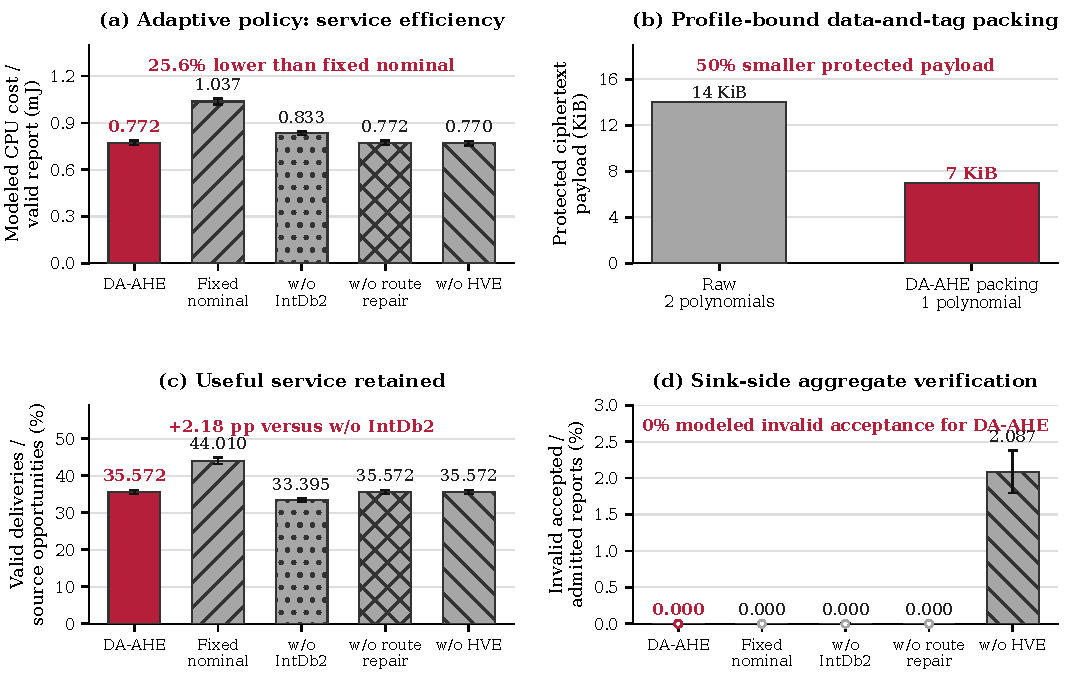
\includegraphics[width=\textwidth]{figures/revised-ablationA.pdf}
\caption{DA-AHE component contributions at 3,000 source nodes. (a) Modeled CPU cost per valid report, normalized within each seed; (b) protected ciphertext payload for raw two-polynomial and packed one-polynomial representations at fixed rank 6; (c) valid delivery per source opportunity; (d) modeled invalid acceptance per admitted report. Bars in (a), (c) and (d) show equally weighted means over 20 paired seeds; error bars are pointwise 95\% percentile-bootstrap intervals from 100,000 shared seed resamples. Panel (b) is exact payload accounting and excludes tickets, MACs, headers and retransmissions. Fixed nominal is the without-Markov policy; its admission rate differs from DA-AHE, so panel (a) compares complete policies. Route-repair and full DA-AHE outcomes coincide in this archive. All recovery records are right-censored; no recovery-time ranking is shown. Modeled invalid acceptance does not estimate a cryptographic forgery probability.}
\label{fig:ablation}
\end{figure*}
